% quickstart.tex
% 电磁场与微波实验报告快速开始
% 请将本文件的内容复制到所要编写的实验报告，不要直接改动、编译此文件！
\documentclass{../ElectromagneticFieldTemplate}

% ====== 额外需要的宏包 ======
\usepackage{subcaption}   % 用于子图排列
\usepackage{float}        % 固定图片位置

% ====== 图片路径设置 ======
% 请将 BUPT 和 badge 两个图片文件（无需扩展名，或实际为 .png/.jpg）放在 ./TemplateFigures/ 目录下
% 如果图片文件有扩展名（如 .png），请使用 
\includegraphics[width=6cm]{BUPT.png}
\graphicspath{{./Figures/}{../TemplateFigures/}}

% ====== 填写实验基本信息 ======
% 顺序：{实验名称}{班级}{姓名}{学号}{指导老师}{日期}
\setExperimentInfo
    {光纤通信系统仿真实验}
    {2024217802}
    {严子竣}
    {2024212622}
    {张璇}
    {\today}              % 自动生成当前日期，也可手动写“2026年5月”

\begin{document}

% 生成封面（包含页眉）
\maketitle

% ========== 以下为正文，章节序号自动为“一、二、…” ==========

\section{实验目的}

\begin{enumerate}
    \item 掌握光纤通信系统的仿真方法，理解强度调制-直接检测（IM-DD）系统的结构。
    \item 研究色散（GVD）和非线性效应（自相位调制 SPM）对光脉冲传输的影响。
    \item 学习使用色散补偿光纤（DCF）进行色散管理，并利用眼图及 Q 因子评估系统性能。
    \item 熟练使用 MATLAB 实现非线性薛定谔方程的分步傅里叶法求解。
\end{enumerate}

\section{实验原理与说明}

\subsection{光纤传输的数学描述}
光脉冲在光纤中的传输服从非线性薛定谔方程（NLSE）：
\[
\frac{\partial A}{\partial z} + \frac{\alpha}{2} A + \frac{\mathrm{i}}{2}\beta_2 \frac{\partial^2 A}{\partial T^2} = \mathrm{i}\gamma |A|^2 A
\]
其中 \(A\) 为慢变包络，\(\beta_2\) 表示色散系数，\(\gamma\) 为非线性系数，\(\alpha\) 为损耗系数。

\subsection{色散与非线性效应}
\begin{itemize}
    \item \textbf{色散（GVD）}：不同频率成分传播速度不同，导致脉冲展宽。展宽程度与传输距离成正比。
    \item \textbf{自相位调制（SPM）}：高功率下折射率随光强变化，产生非线性相移，引起频率啁啾，导致频谱展宽。
    \item \textbf{色散补偿}：利用负色散系数光纤（DCF）抵消正色散，使总色散为零。
\end{itemize}

\subsection{性能评估指标}
\begin{itemize}
    \item \textbf{眼图}：观察码间串扰和噪声容限。
    \item \textbf{Q 因子}：反映信噪比，Q 值越大误码率越低。最佳抽样时刻即 Q 最大值对应的时刻。
\end{itemize}

\section{实验设备}

\begin{enumerate}
    \item 安装MATLAB R2023a的电脑
    \item 仿真程序 \texttt{GVDSPM.m}（含分步傅里叶法、贝塞尔滤波、眼图分析等模块）
\end{enumerate}

\section{实验内容}

本实验通过修改 \texttt{GVDSPM.m} 中的入纤功率 \(P_{0dB}\) 和传输距离 \(L_{smf}\)（并相应调整 DCF 长度 \(L_{dcf}\) 使总色散抵消），对比 5 种典型情况下的信号传输质量：
\begin{enumerate}
    \item 低功率（0 dBm）+ 短距离（40 km）
    \item 低功率（0 dBm）+ 中距离（80 km）
    \item 低功率（0 dBm）+ 长距离（120 km）
    \item 中功率（5 dBm）+ 中距离（80 km）
    \item 高功率（10 dBm）+ 中距离（80 km）
\end{enumerate}
观察发射端、SMF 后、DCF 后及接收端各点的时域波形、光谱、眼图及 Q 因子曲线，分析色散与非线性对系统性能的影响。

\section{实验步骤}

\begin{enumerate}
    \item 运行 \texttt{GVDSPM.m}；将16张图片合成一张大图并按类别调整子图顺序。
    \item 依次修改代码中的参数：
    \begin{itemize}
        \item \texttt{P0dB}：0, 5, 10
        \item \texttt{L\_smf}：40e3, 80e3, 120e3
        \item \texttt{L\_dcf}：按比例调整，保持总色散为零（例如 8e3, 16e3, 24e3）。
    \end{itemize}
    \item 读取眼图并记录 Q 因子最大值及对应时刻。
    \item 对比不同参数下的波形变化。
\end{enumerate}

\section{实验数据}

以下展示了 5 种参数配置下的完整仿真结果（含时域波形、光谱、眼图及 Q 因子曲线），每张图采用 4×4 网格排列。

\begin{figure}[H]
    \centering
    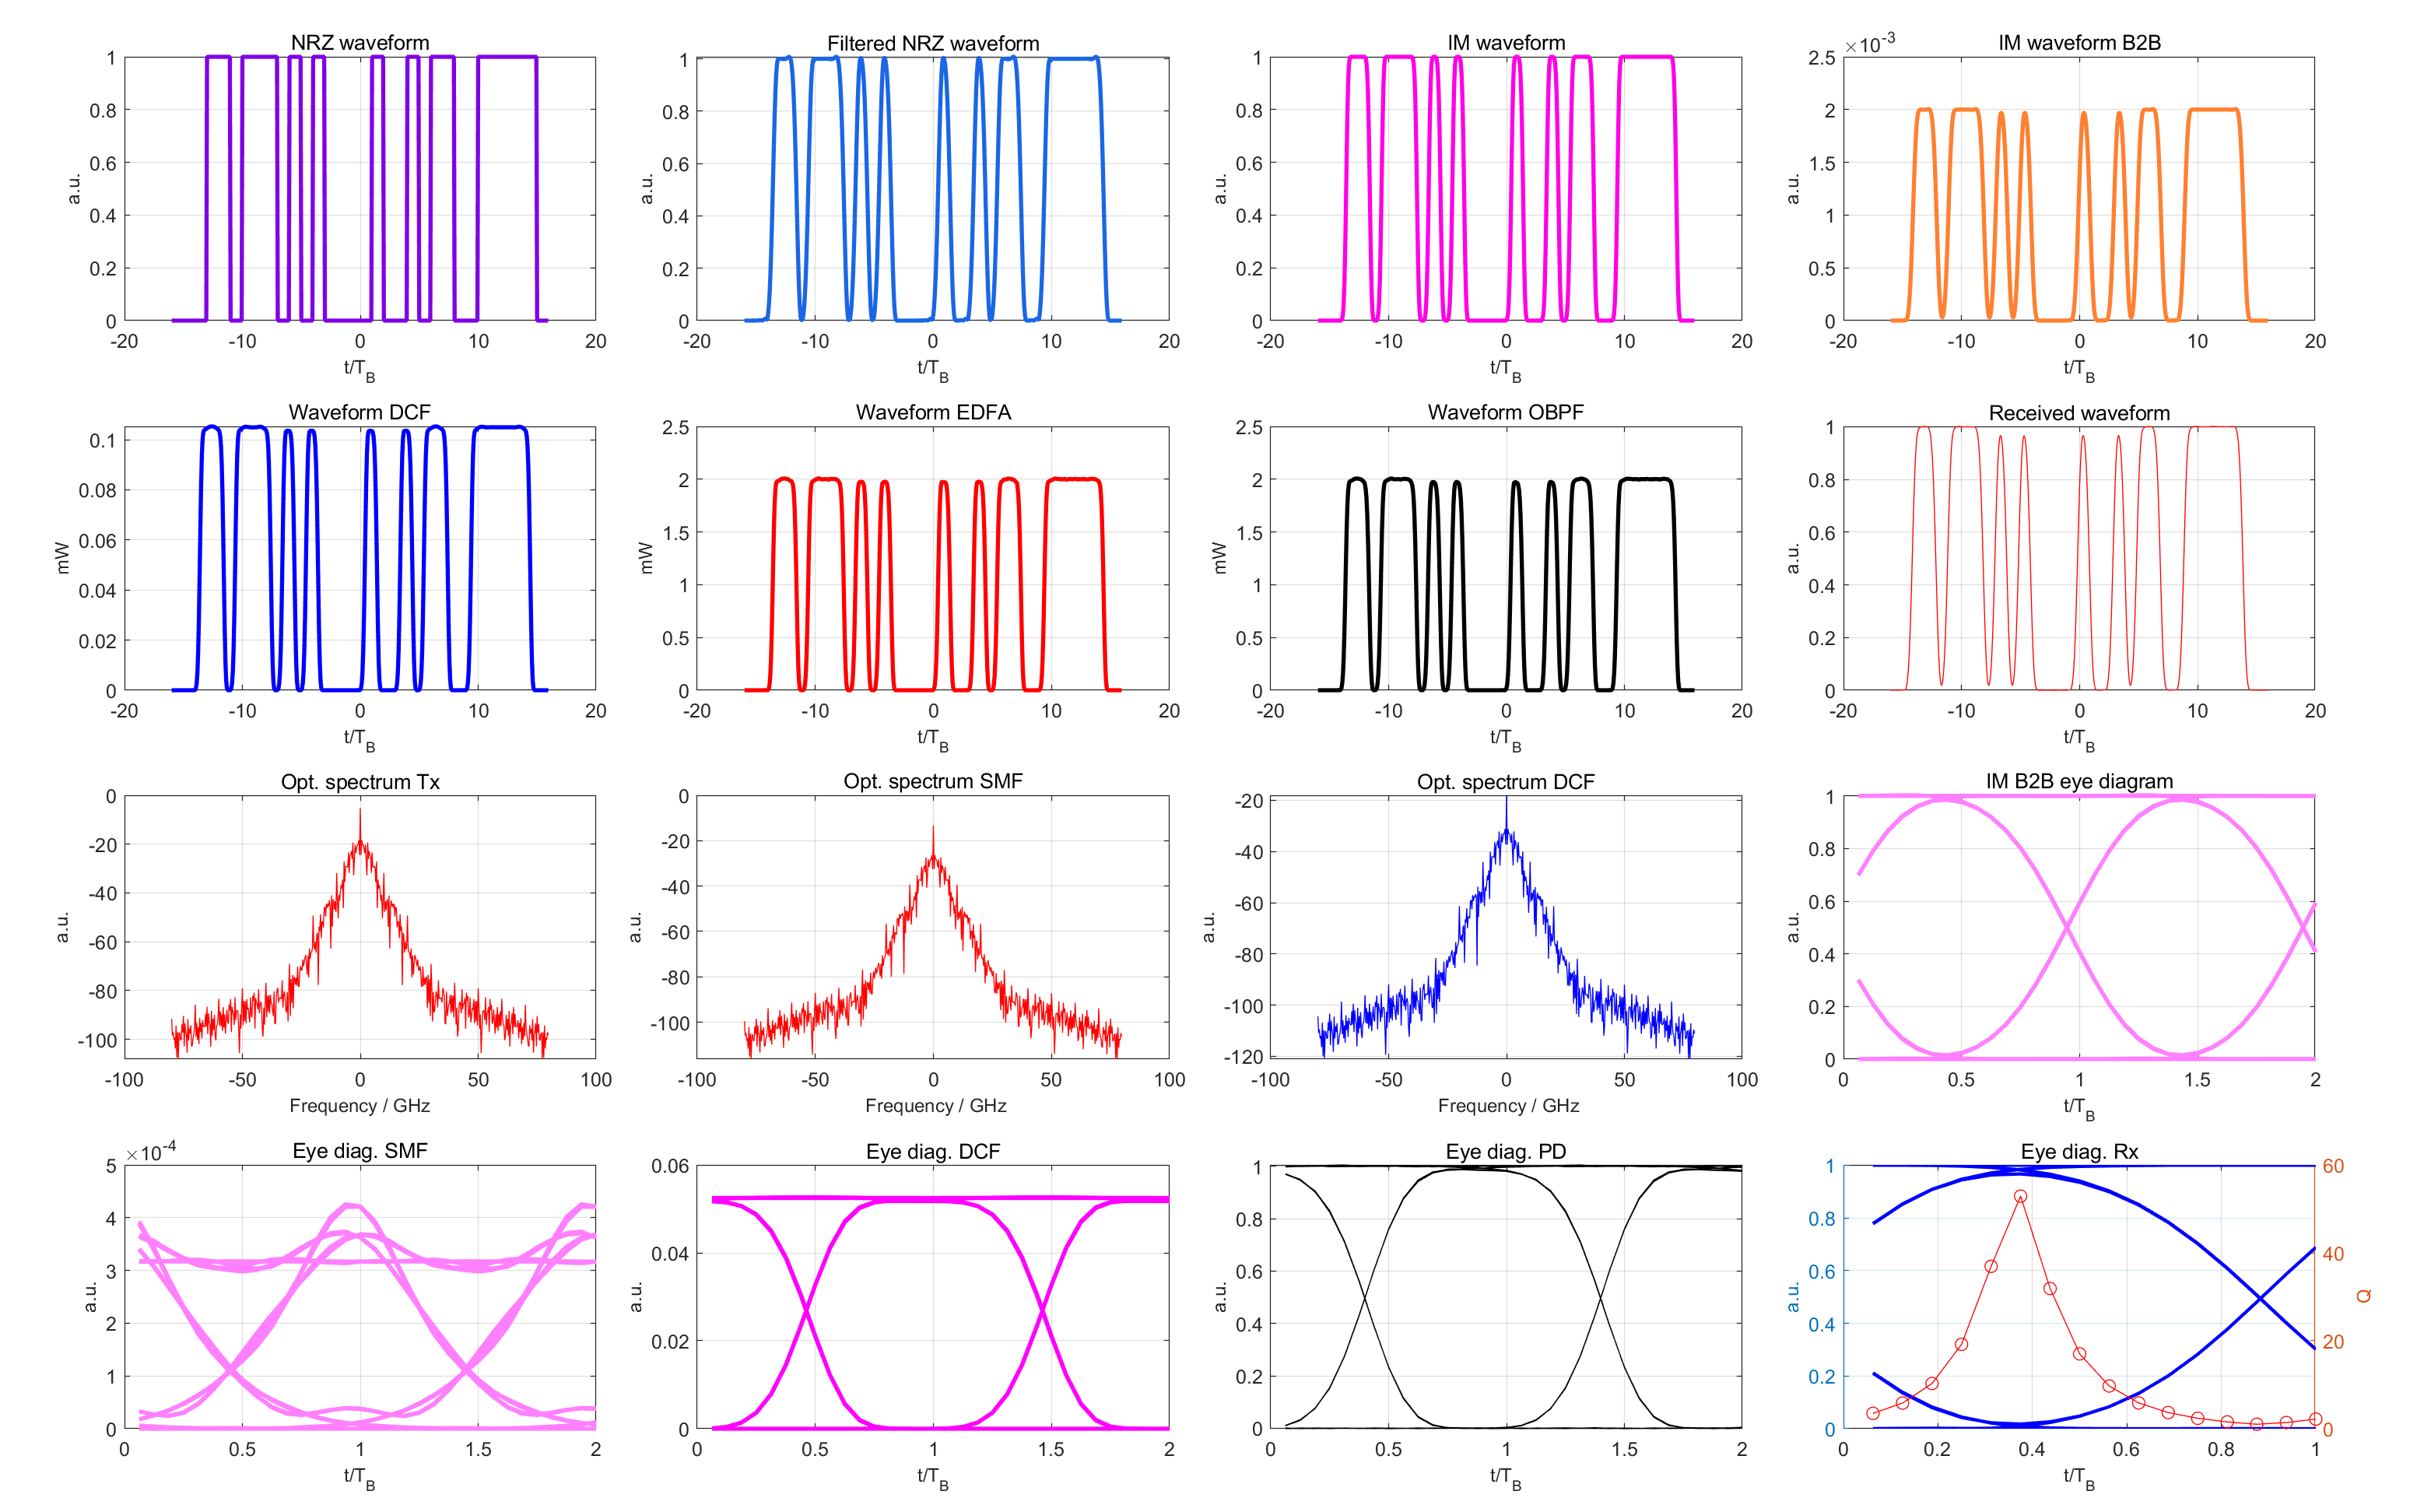
\includegraphics[width=0.95\linewidth]{LowPowerLowDistance.png}
    \caption{低功率（0 dBm）+ 短距离（40 km）仿真结果}
    \label{fig:low_power_low_dist}
\end{figure}

\begin{figure}[H]
    \centering
    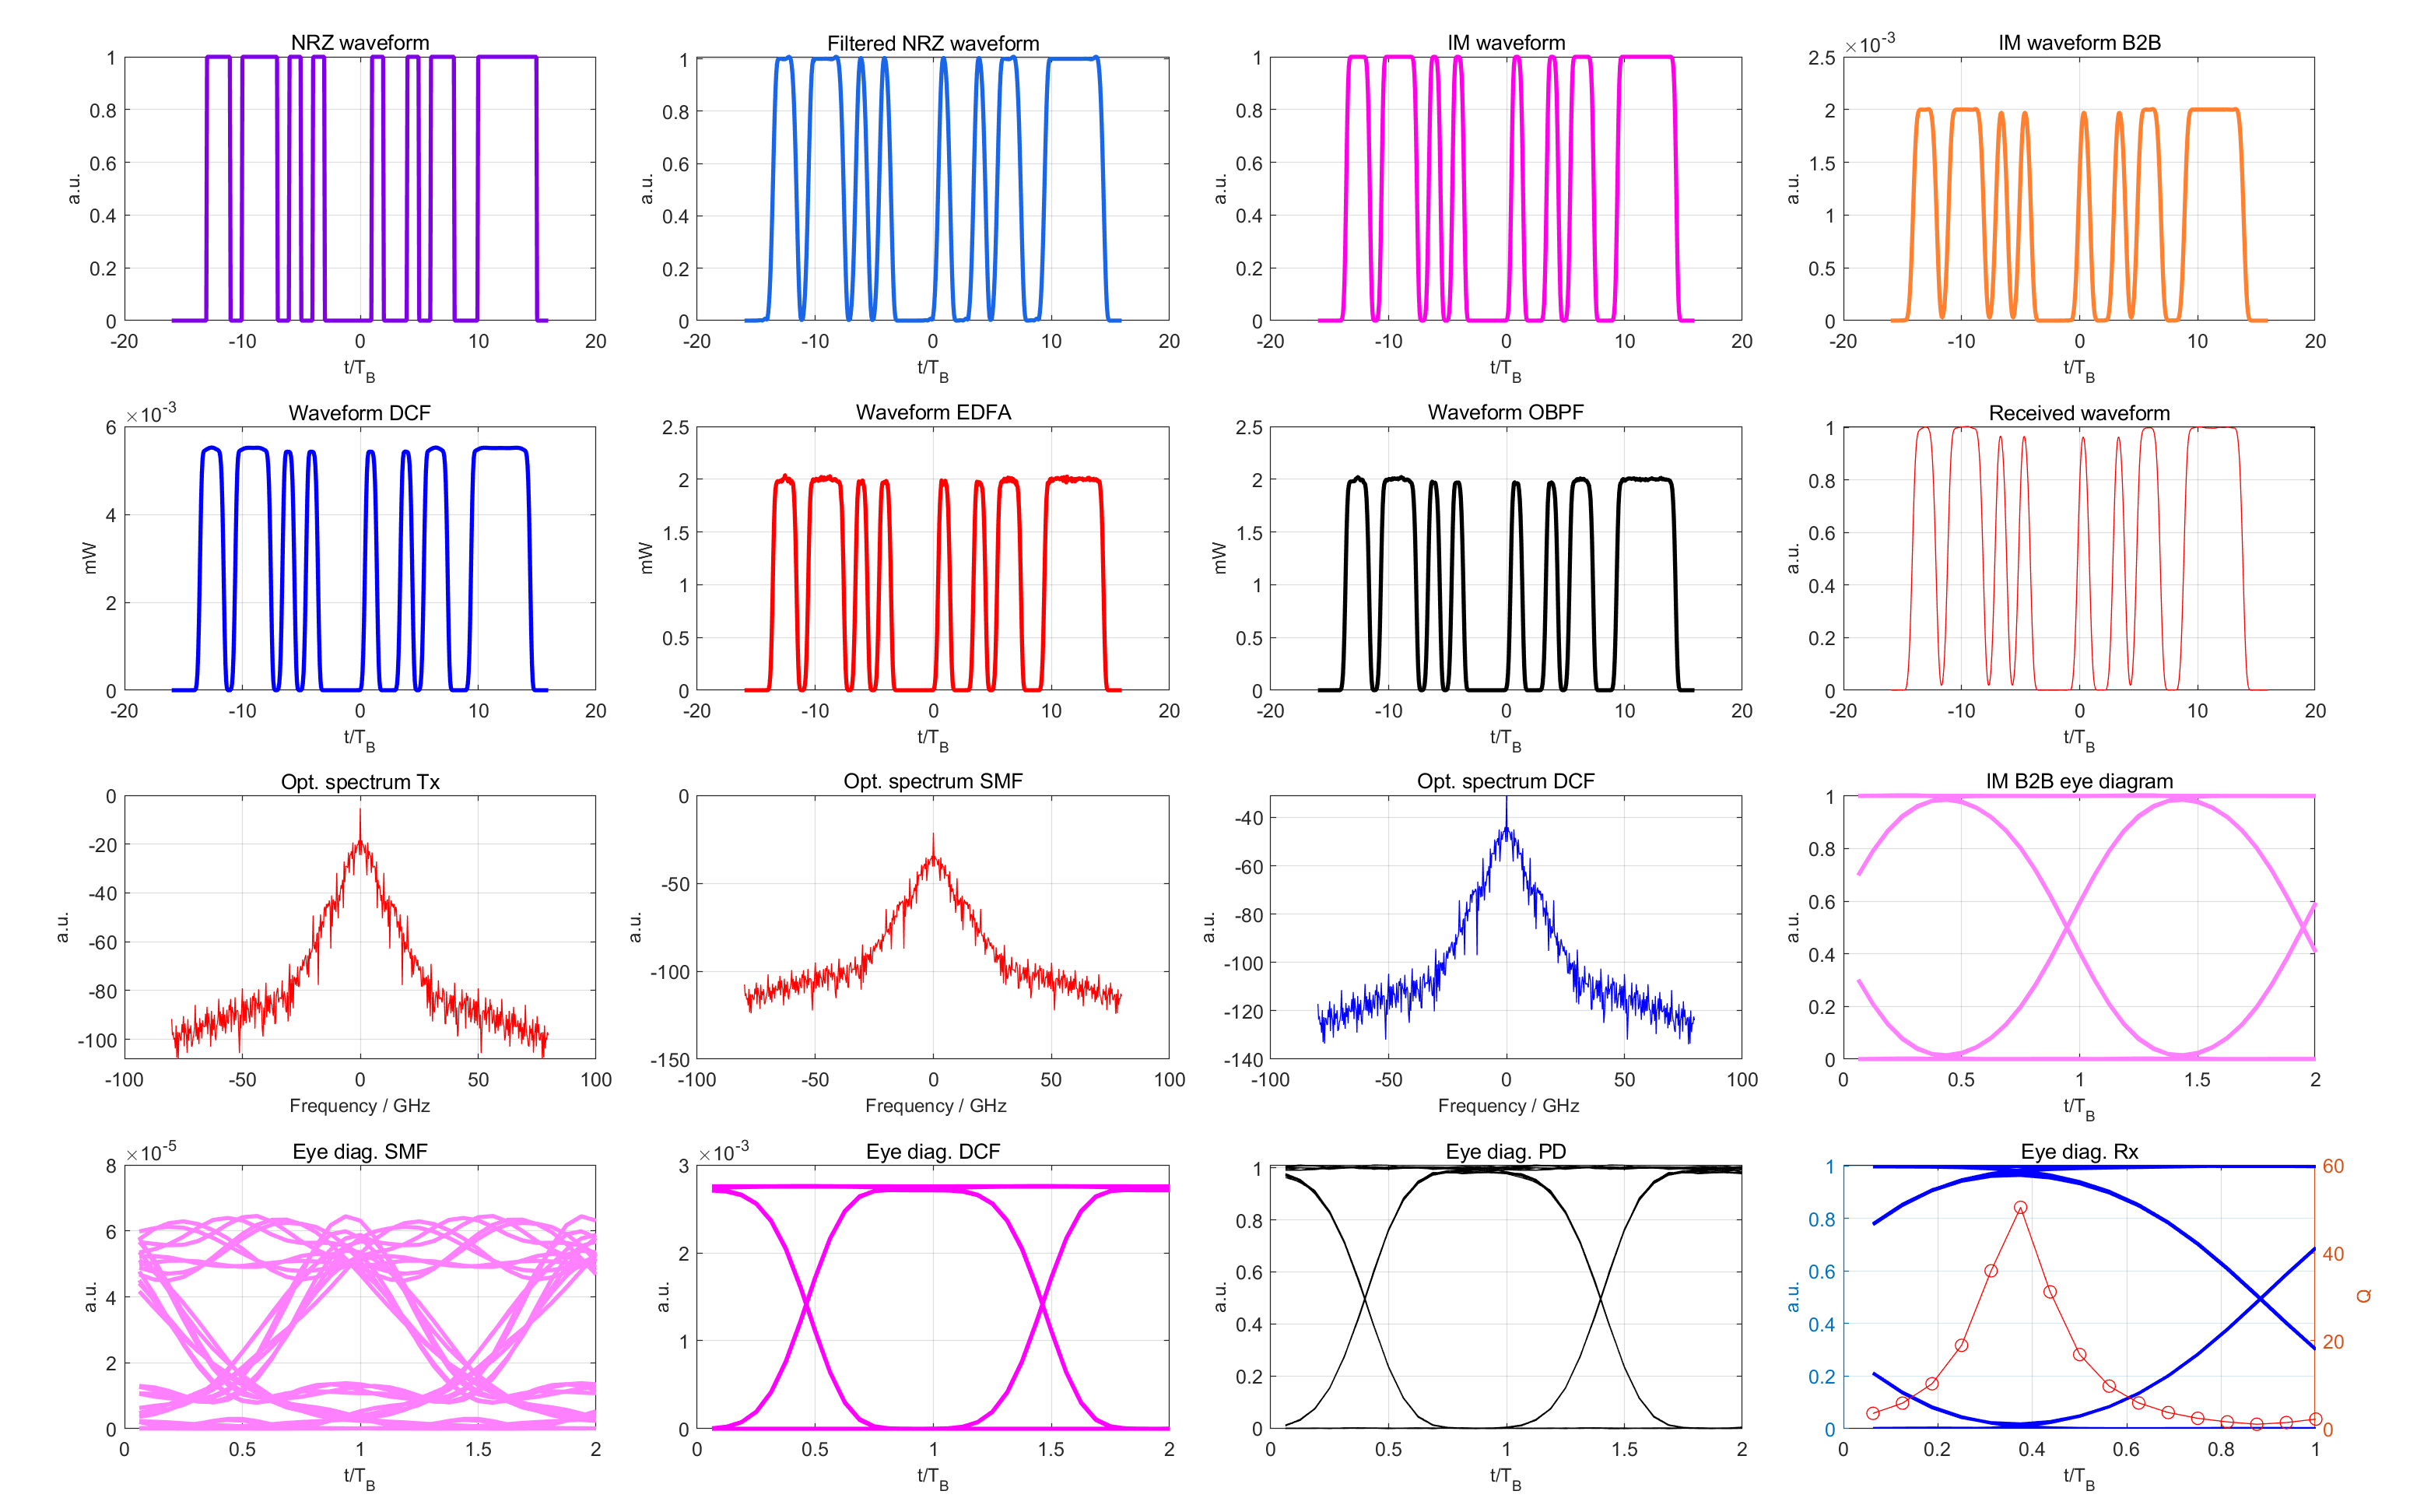
\includegraphics[width=0.95\linewidth]{LowPowerMedDistance.png}
    \caption{低功率（0 dBm）+ 中距离（80 km）仿真结果}
    \label{fig:low_power_med_dist}
\end{figure}

\begin{figure}[H]
    \centering
    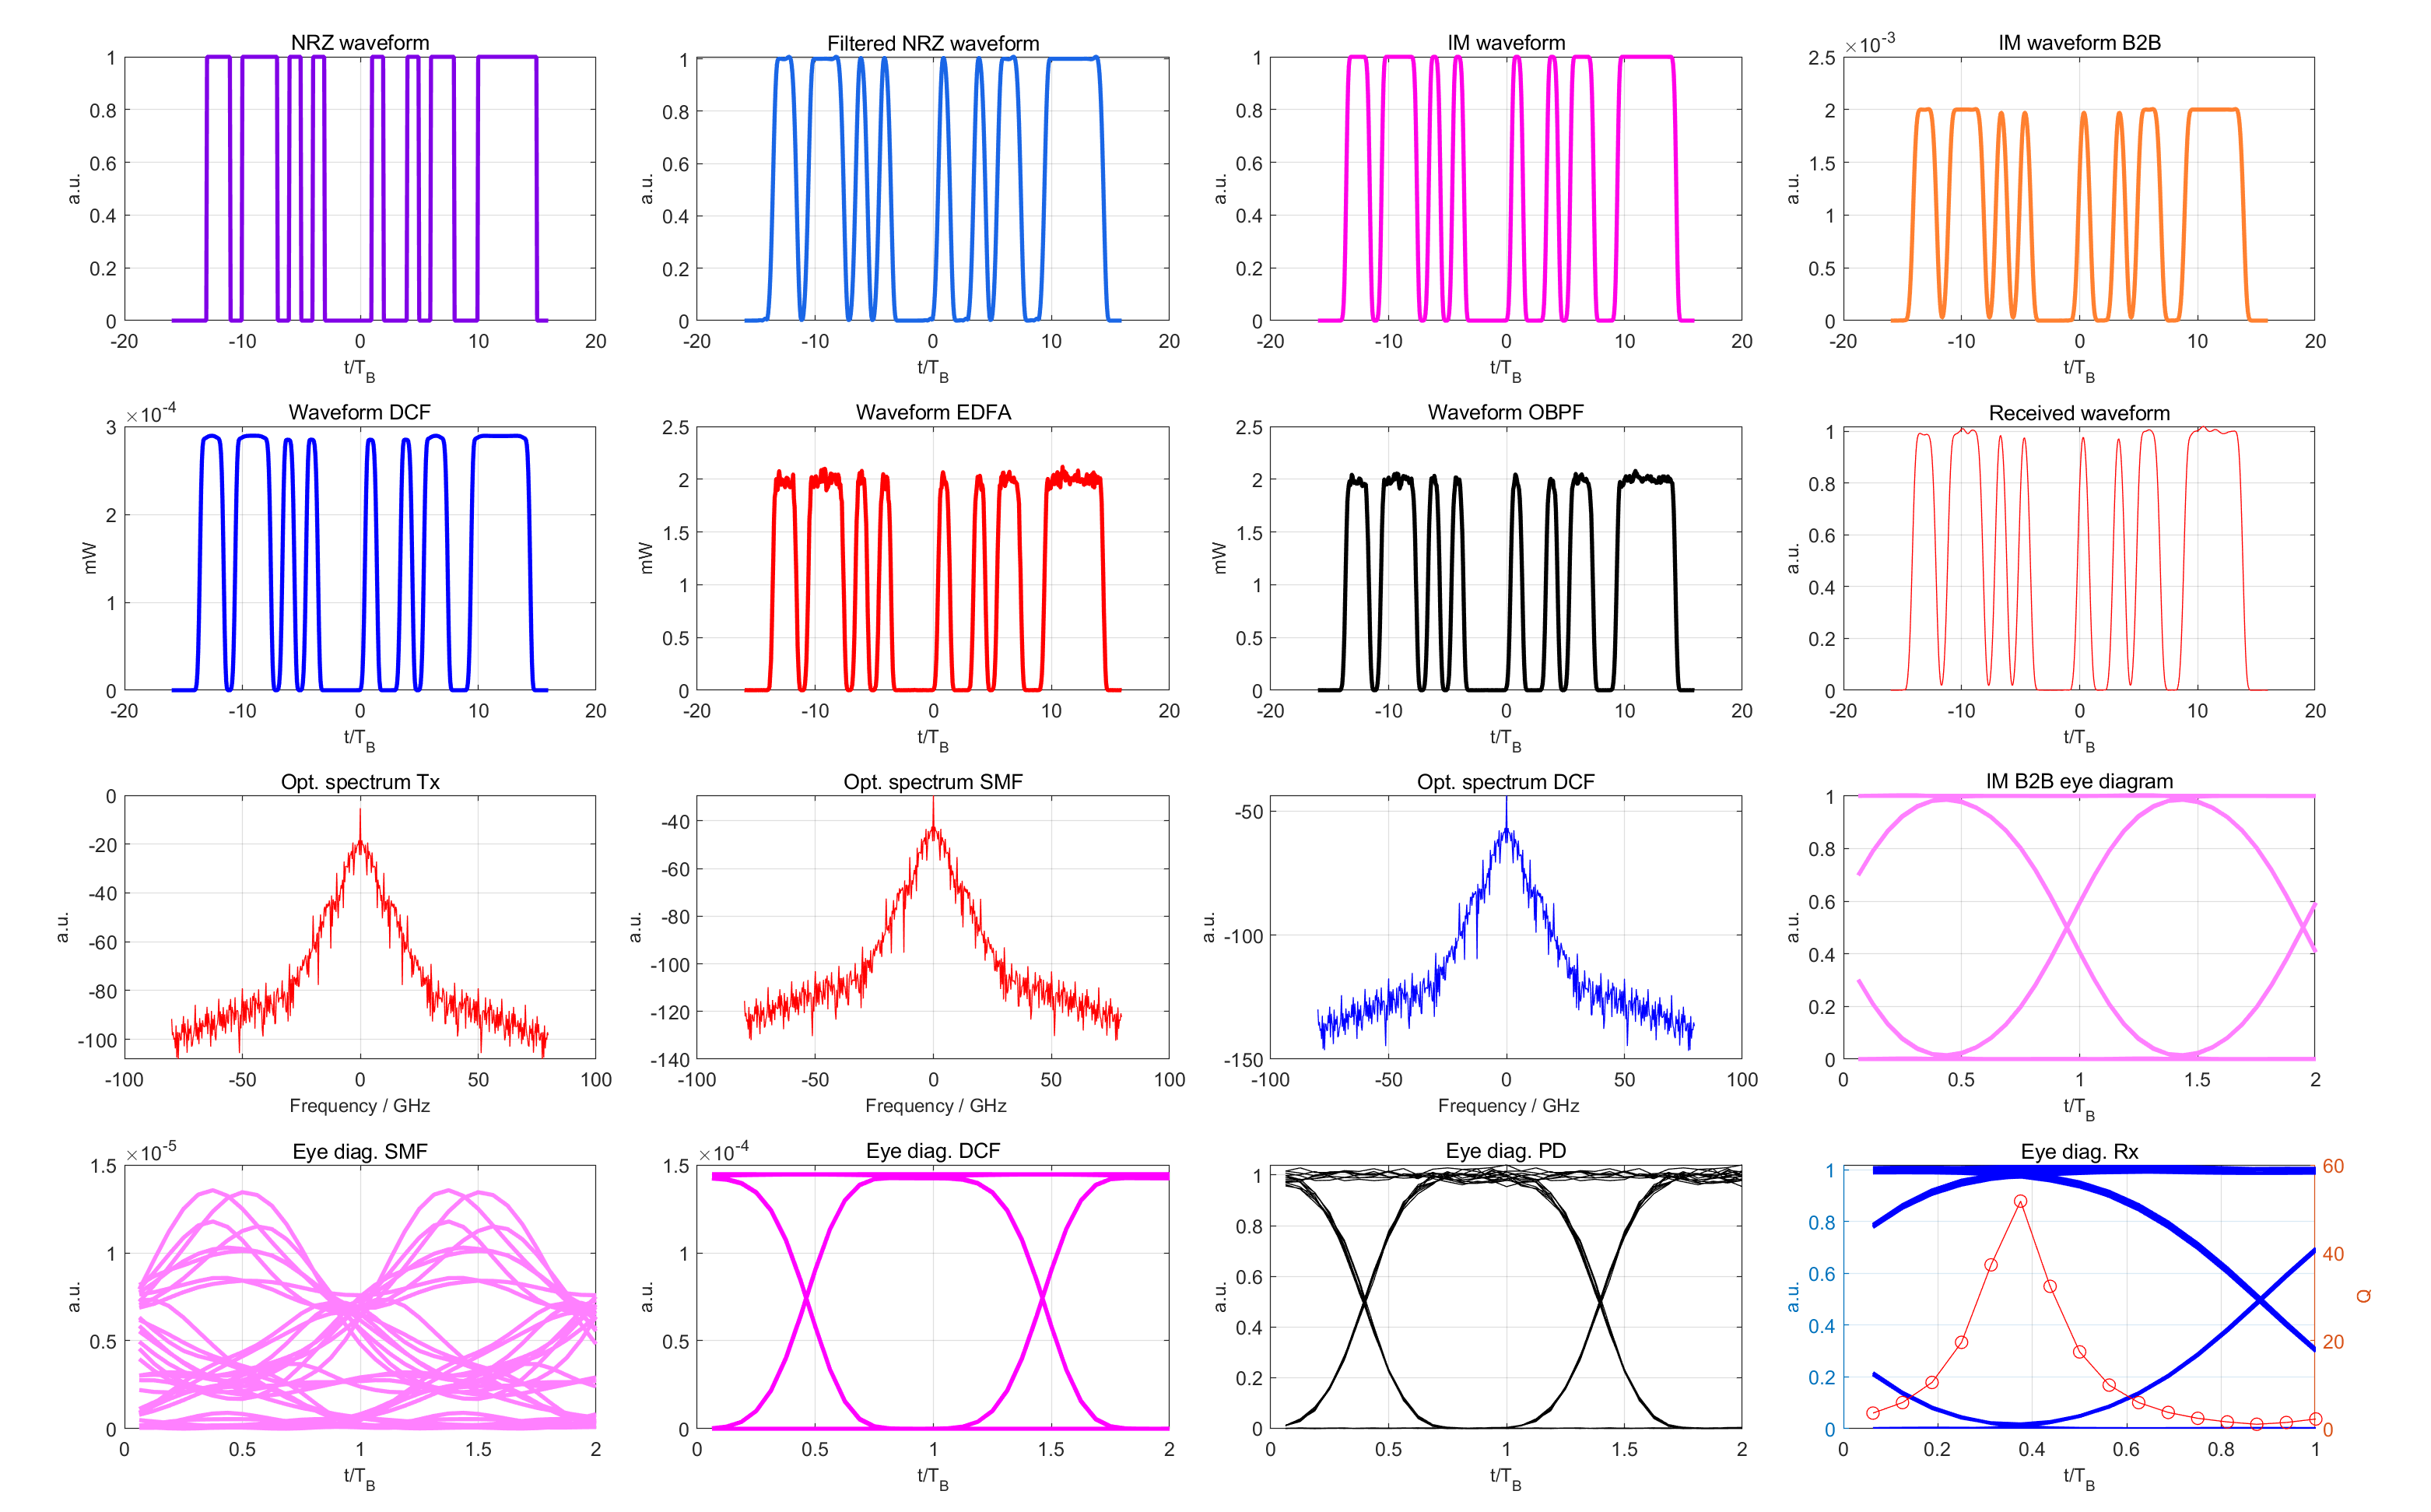
\includegraphics[width=0.95\linewidth]{LowPowerHighDistance.png}
    \caption{低功率（0 dBm）+ 长距离（120 km）仿真结果}
    \label{fig:low_power_high_dist}
\end{figure}

\begin{figure}[H]
    \centering
    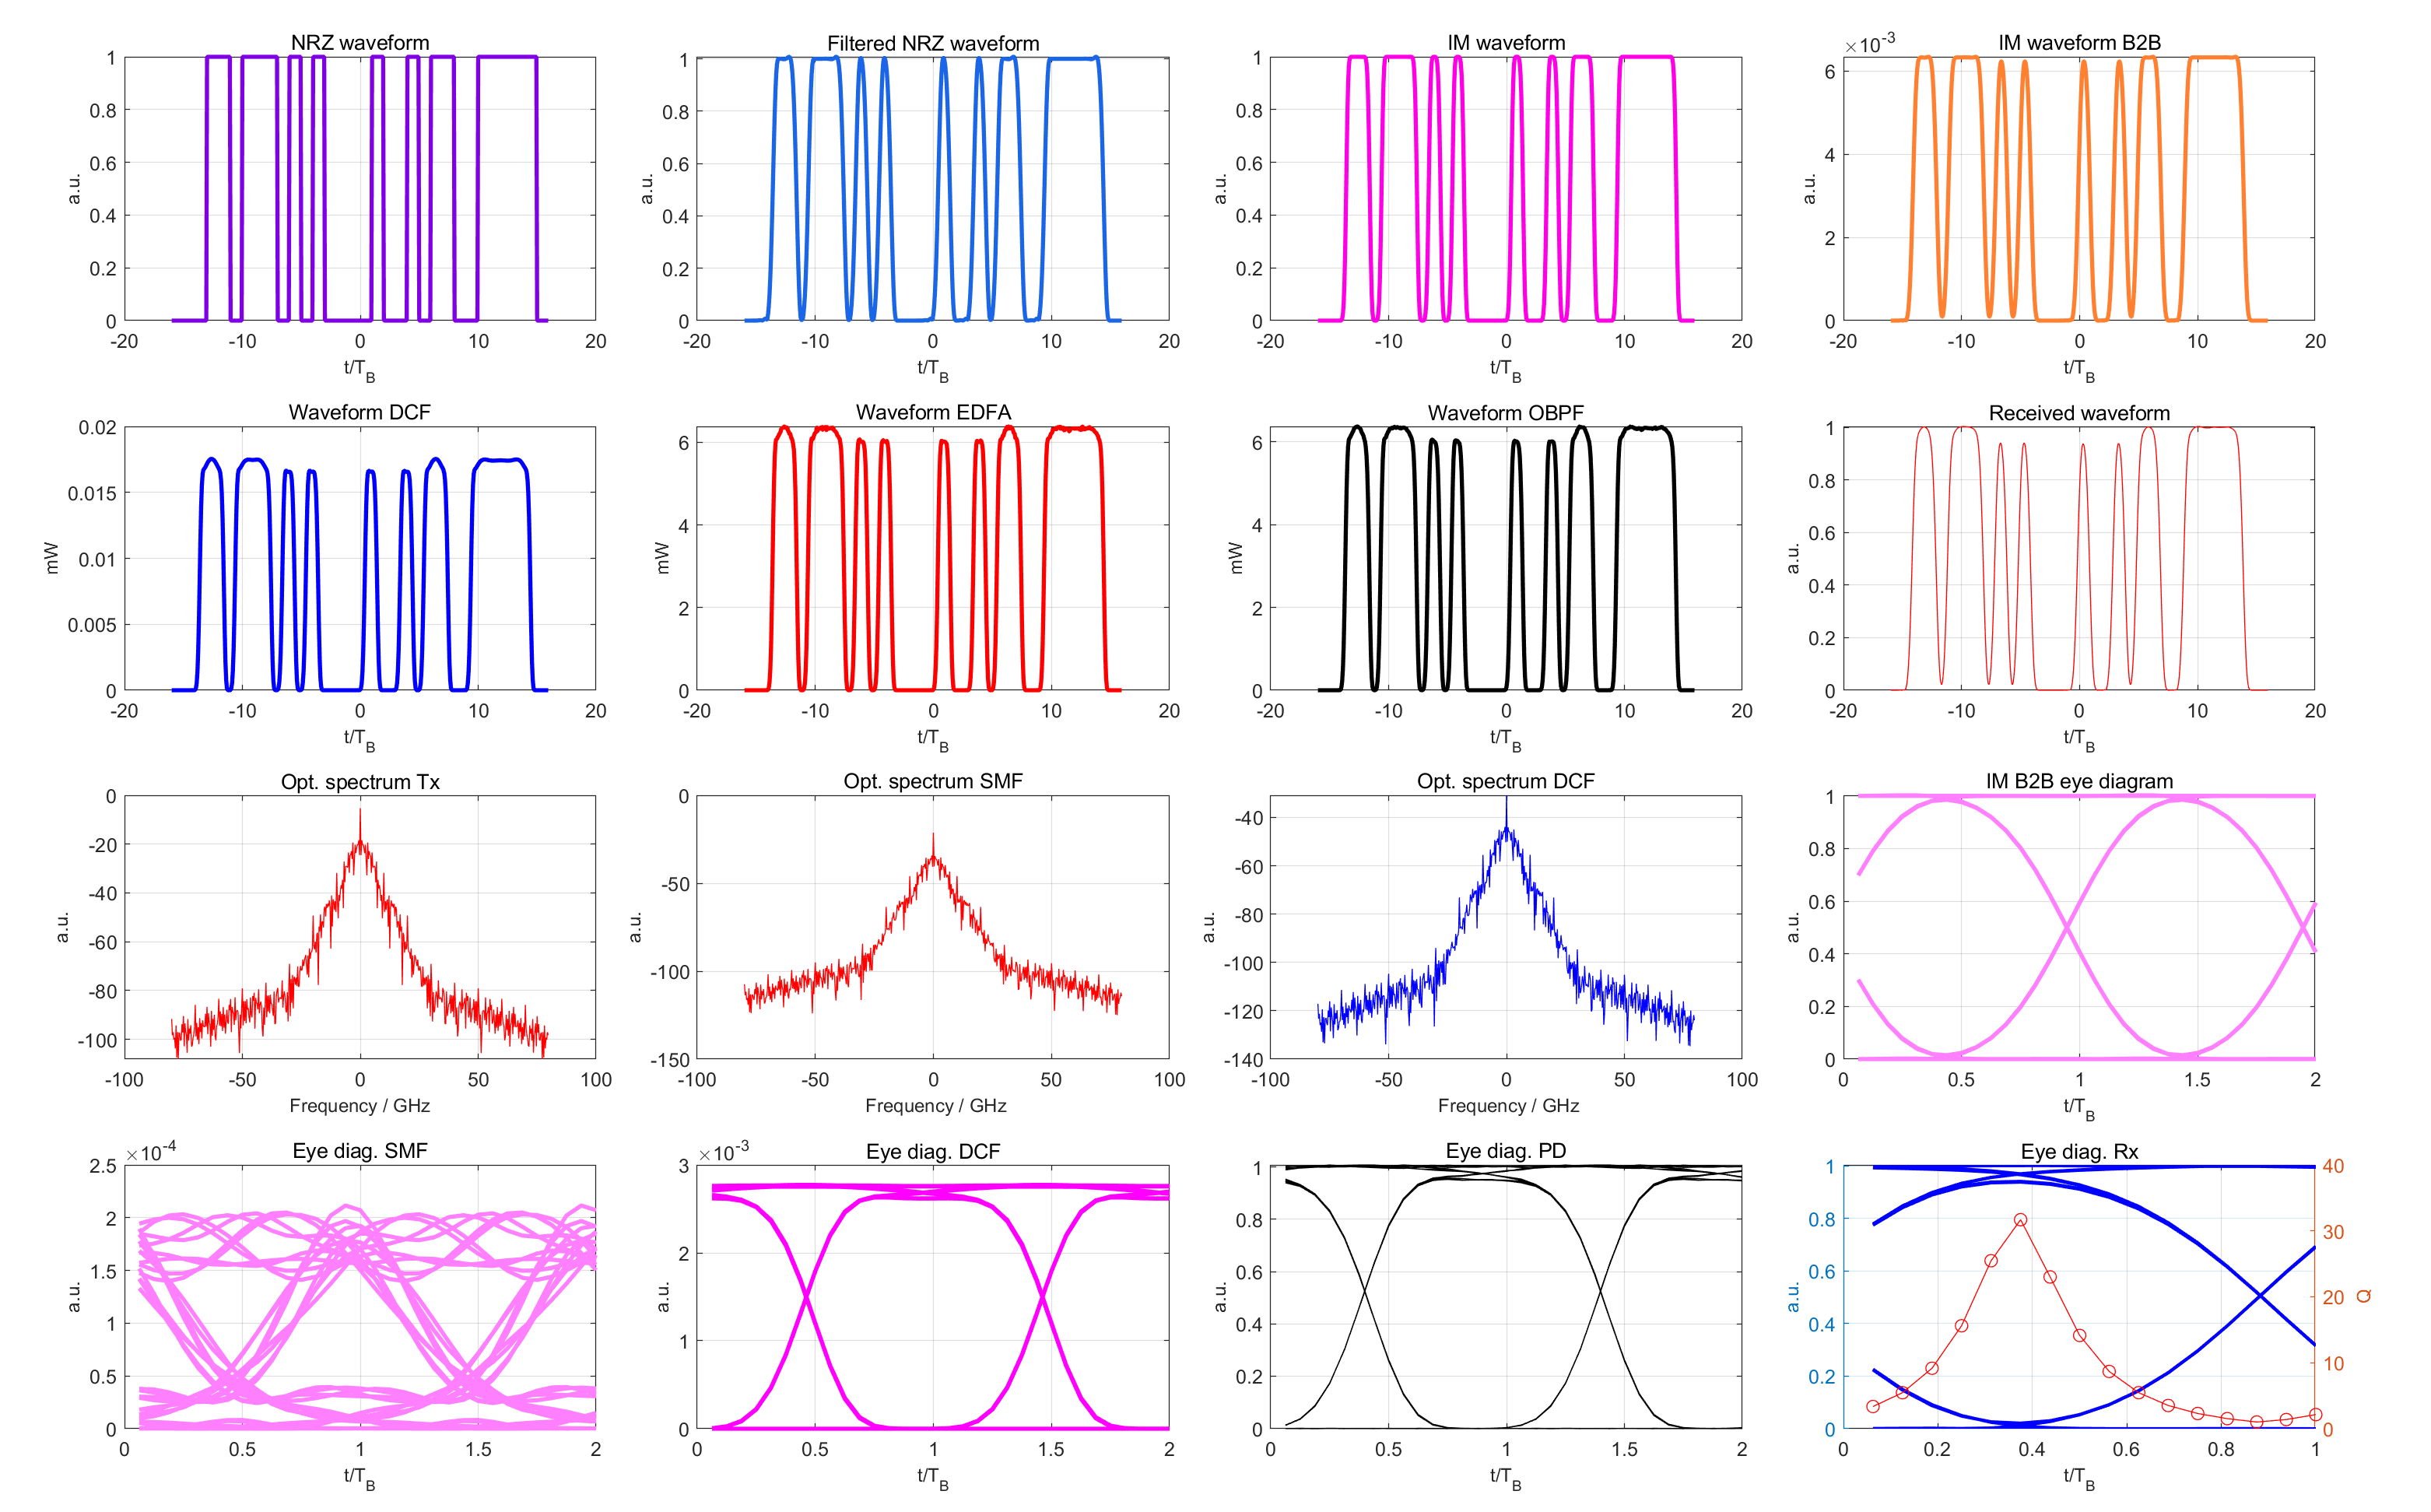
\includegraphics[width=0.95\linewidth]{MedPowerMedDistance.png}
    \caption{中功率（5 dBm）+ 中距离（80 km）仿真结果}
    \label{fig:med_power_med_dist}
\end{figure}

\begin{figure}[H]
    \centering
    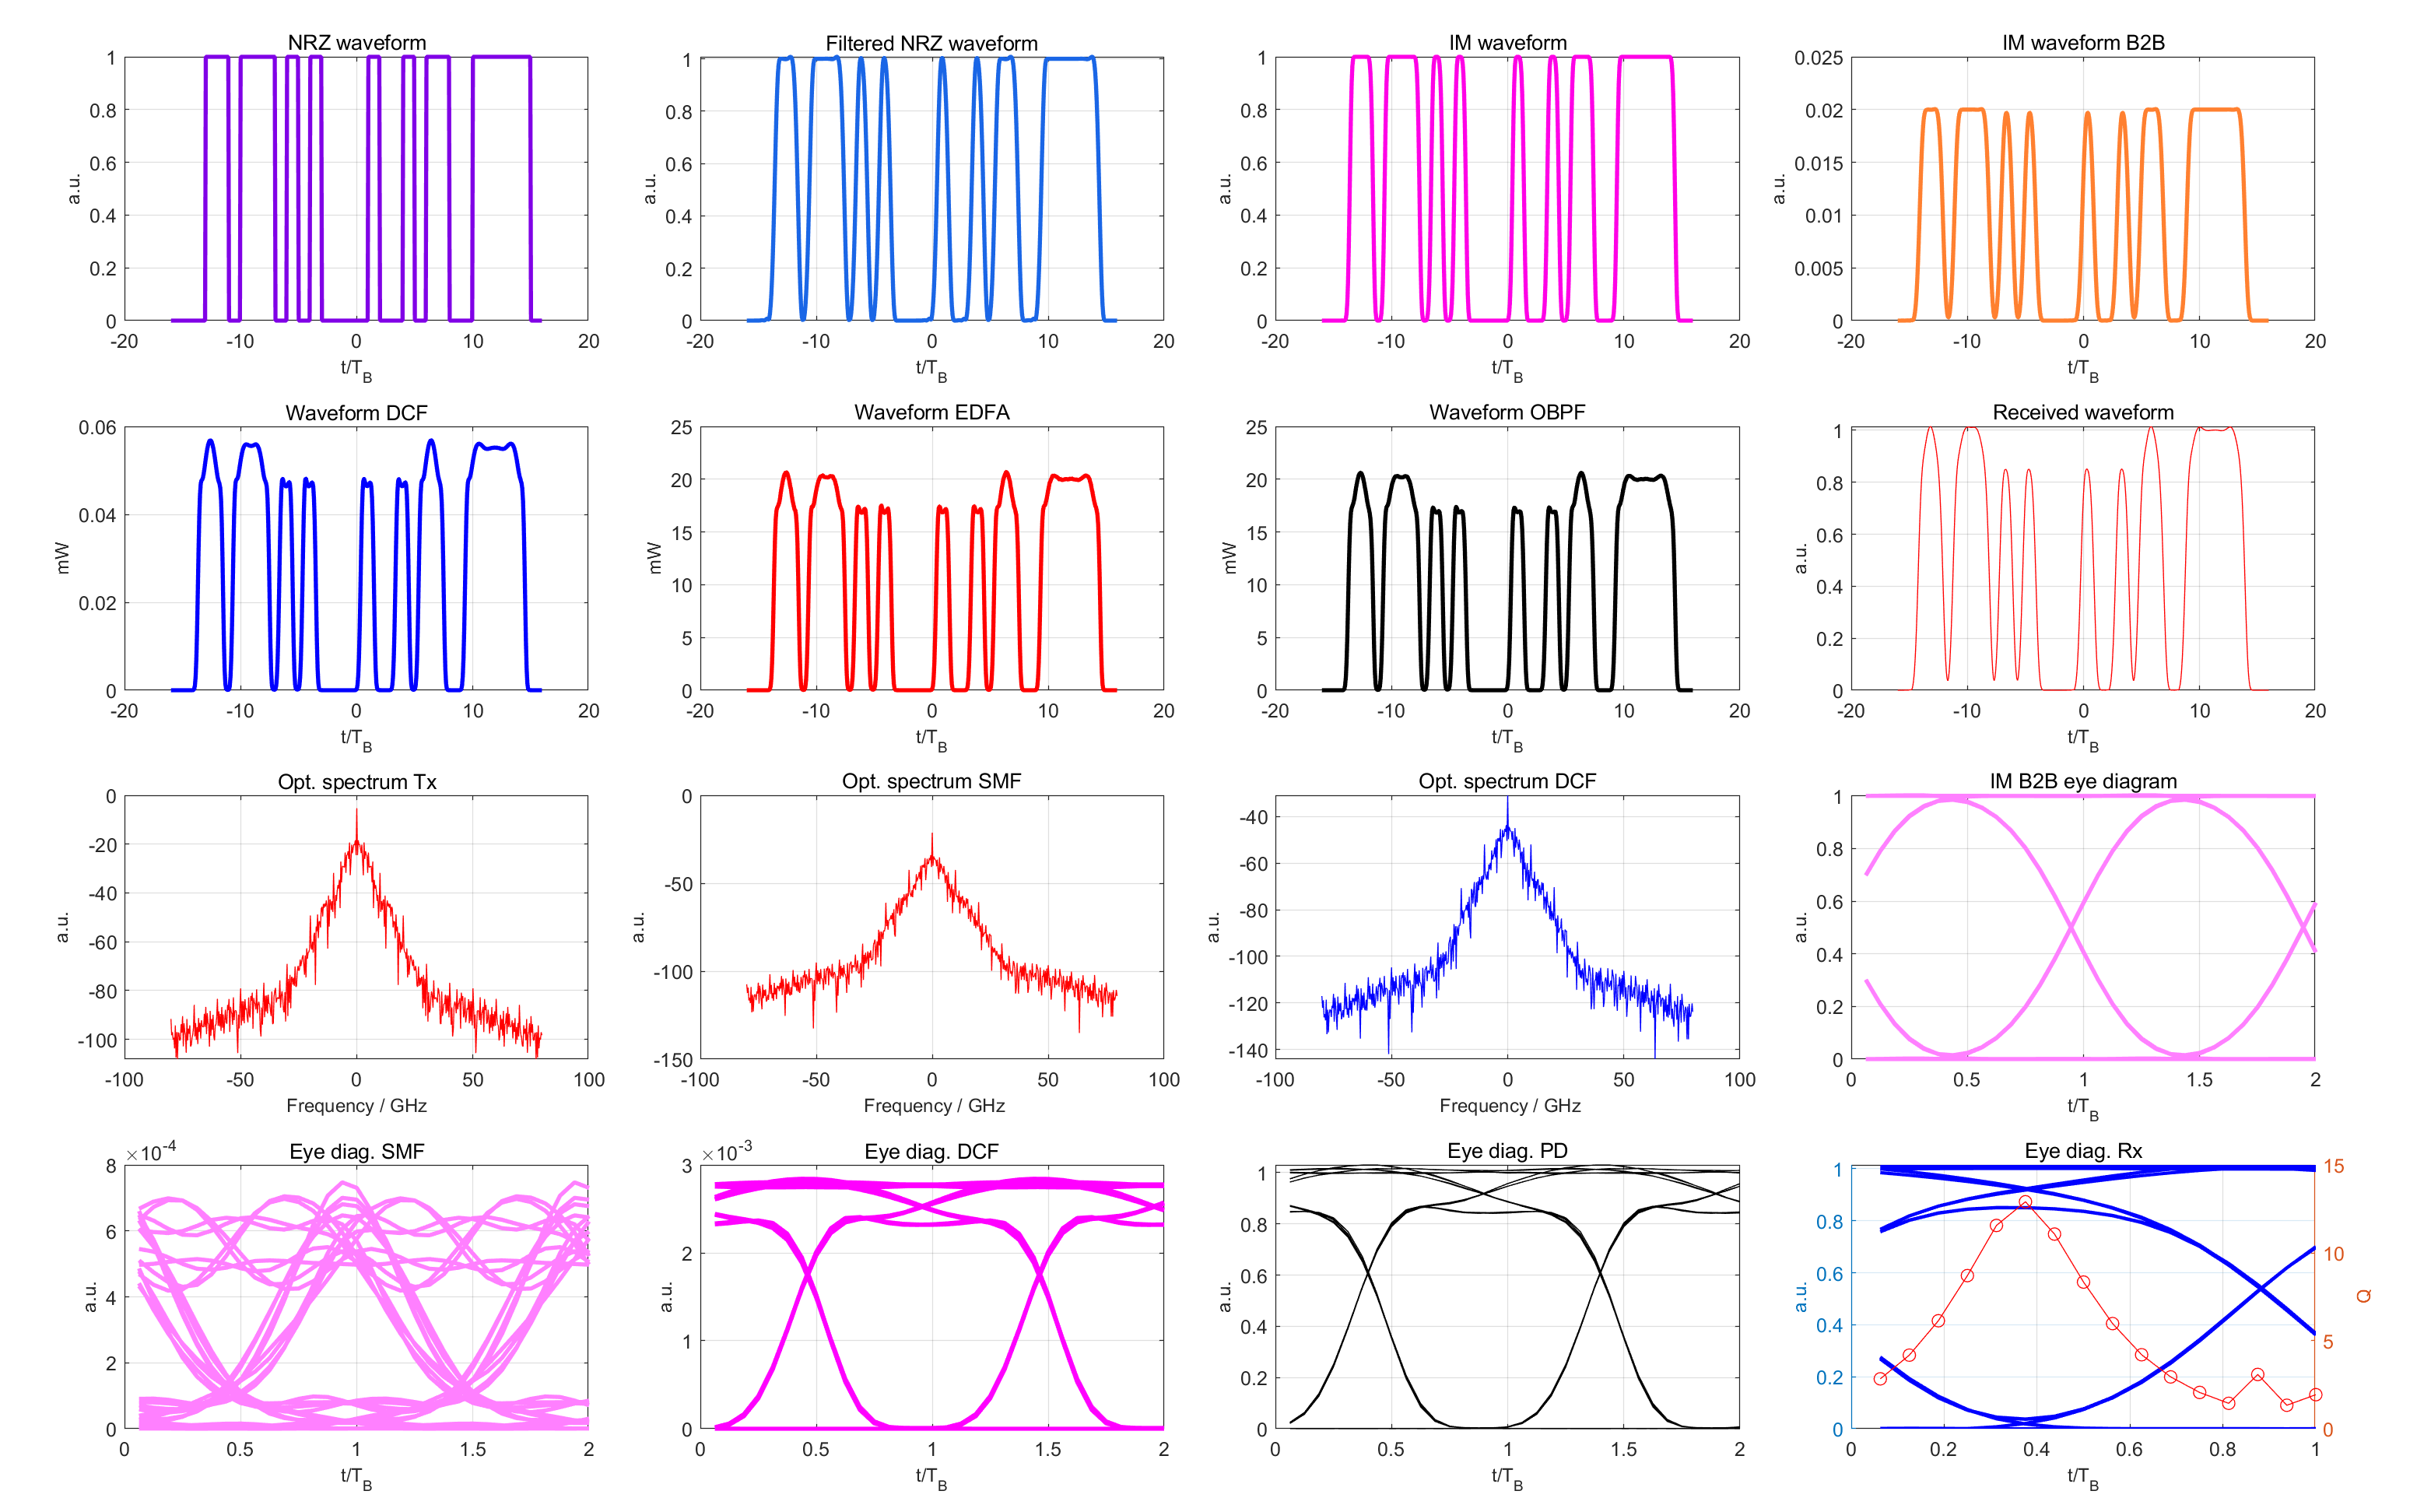
\includegraphics[width=0.95\linewidth]{HighPowerMedDistance.png}
    \caption{高功率（10 dBm）+ 中距离（80 km）仿真结果}
    \label{fig:high_power_med_dist}
\end{figure}

\section{实验结果整理及误差分析}

\subsection{色散的影响（低功率组）}
从图 \ref{fig:low_power_low_dist}、\ref{fig:low_power_med_dist} 和 \ref{fig:low_power_high_dist} 可见，当入纤功率较低（非线性可忽略）时，色散是主要损伤因素。
\begin{itemize}
    \item 随着传输距离从 40 km 增加到 120 km，SMF 输出眼图（各图中第 3 行第 1 列）的“眼睛”明显闭合，脉冲宽度展宽。
    \item 色散补偿后（DCF 输出眼图，第 3 行第 2 列），眼图重新张开，证明色散补偿有效。
    \item 接收端 Q 因子随距离增加而下降，但经补偿后仍能保持一定性能。
\end{itemize}

\subsection{非线性的影响}
对比图 \ref{fig:low_power_med_dist} 与 \ref{fig:med_power_med_dist}（中距离 80 km，功率从 0 dBm 增加到 5 dBm）：
\begin{itemize}
    \item 光谱（第 2 行第 1 列）出现轻微展宽，表明 SPM 产生了频率啁啾。
    \item 眼图（第 3 行第 4 列）的 Q 因子略有提升（约 15 → 30），这是因为在反常色散区，SPM 引起的正啁啾与色散相互作用，初期可产生脉冲压缩效应，暂时改善信号质量。
\end{itemize}

\subsection{高功率下的非线性损伤}
图 \ref{fig:high_power_med_dist} 显示了高功率（10 dBm）下的结果：
\begin{itemize}
    \item 光谱展宽显著（第 2 行第 1 列），能量向边带分散。
    \item 眼图呈现明显的“抖动”和不对称（第 3 行第 4 列），Q 因子反而下降（约 40），说明过高的非线性导致信号严重劣化。
    \item 时域波形（第 2 行第 2 列）的峰值波动增大，码间串扰加剧。
\end{itemize}

\subsection{误差分析}
\begin{itemize}
    \item 仿真中假设光纤为理想单模，未考虑偏振模色散（PMD）和双折射效应。
    \item 分步傅里叶法的步长（本程序默认 1 km）可能引入数值误差，但已被证明在皮秒脉冲范围内精度足够。
    \item 接收端噪声模型（散粒噪声+热噪声）采用高斯近似，实际光电转换可能存在非线性响应偏差。
    \item 眼图计算中的采样偏差可能影响 Q 因子精确值。
\end{itemize}

\end{document}